\subsubsection{\textit{Câu 2}}

\noindent\textbf{\large Đề bài:} Viết chương trình hợp ngữ cho phép nhập vào một mảng gồm 10 số có hai chữ số. Tính tổng các số chia hết cho 7. In tổng thu được ra màn hình dưới dạng thập phân.

\vspace{0.5cm}
\noindent\textbf{\large Biểu diễn bằng Flowchart:} hình \ref{fig:flowchart-2}

\begin{figure}[H]
    \centering
    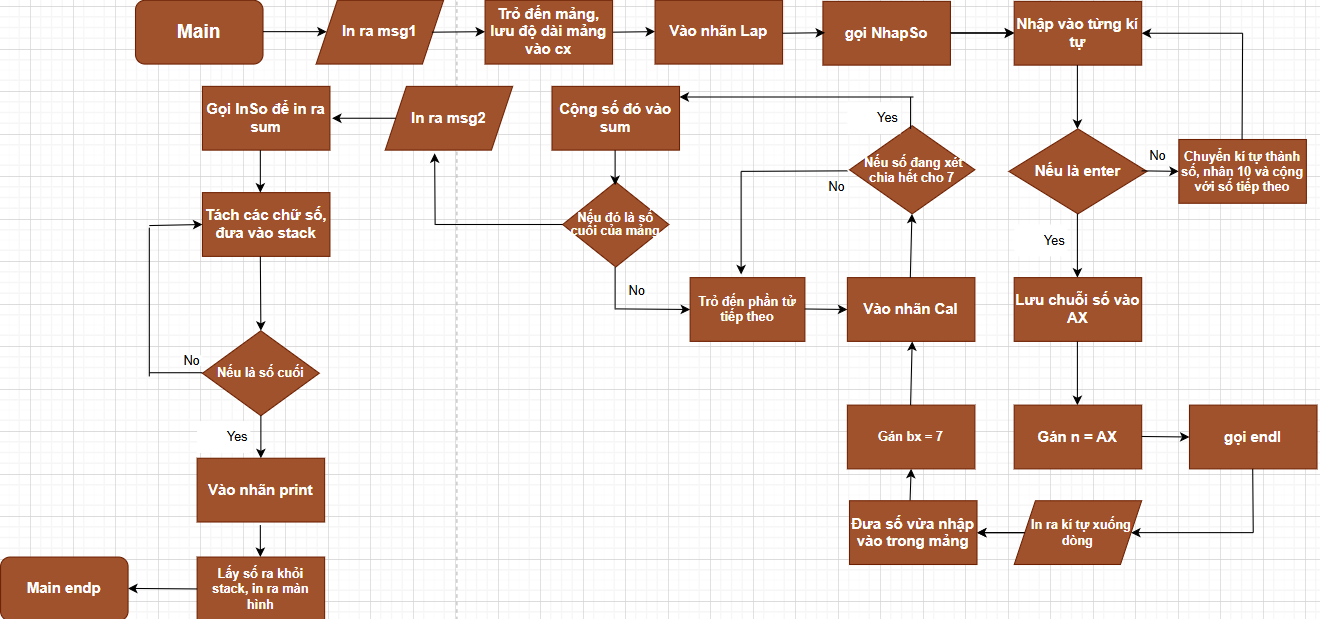
\includegraphics[width=1\textwidth]{Images/Flowchart/Flowchart-2.png}
    \caption{Flowchart tính tổng số chia hết cho 7}
    \label{fig:flowchart-2}
\end{figure}

\vspace{0.5cm}
\noindent\textbf{\large Mã nguồn assembly 8086:}
\begin{lstlisting}[style=asm, caption={Mã nguồn câu 2}]
    .model small               ;Khoi tao che do bo nho la small
    .stack 100                 ;Khoi tao kich thuoc ngan xep
    .data                      ;Khoi tao cac bien
        crlf db 13, 10, '$'                
        x dw ?
        y dw ?              
        sum dw ?
        arr dw 10 dup('$')
        msg1 db 'Nhap 10 so co 2 chu so (moi so tren 1 dong):', 0Dh, 0Ah, '$'
        msg2 db 'Tong cac so chia het cho 7 la: $'
    .code
    main proc                  ;Ham chinh cua chuong trinh
        mov ax, @data
        mov ds, ax             ;Khoi tao thanh ghi ds
        
        mov ah, 9              ;In ra man hinh msg1
        lea dx, msg1
        int 21h
        
        lea si, arr            ;Thanh ghi SI tro den mang arr
        mov cx, 10             ;Luu do dai arr vao thanh ghi cx
        Lap:
            call NhapSo  
            call endl
            mov [si], ax       ;Dua moi so nhap duoc vao trong mang arr
            add si, 2          ;Tang SI tro den phan tu tiep theo cua mang, vi mang dw nen phai +2
            loop Lap           ;Thuc hien nhap mang cho den khi du phan tu
        
        mov cx, 10             ;Luu do dai arr vao thanh ghi cx
        lea si, arr            ;Thanh ghi SI tro den mang arr
        mov bx, 7              ;Luu 7 vao thanh ghi bx 
        Cal:
            mov dx, 0          ;Gan thanh dx = 0
            mov ax, [si]       ;Lay ra tung phan tu dua vao thanh ax
            div bx             ;Lay ax chia bx, phan nguyen luu vao ax, phan du luu vao dx
            cmp dx, 0          ;So sanh dx voi 0
            jne continue       ;Neu dx != 0 thi nhay den continue
            mov ax, [si]       ;Neu dx == 0, tuc la chia het cho 7
            add sum, ax        ;Neu chia het cho 7 thi cong vao sum
            continue:
            add si, 2          ;Tang si tro den phan tu tiep theo
            loop Cal           ;Thuc hien so sanh den phan tu cuoi cung cua mang
        
        mov ah, 9              ;In ra msg2
        lea dx, msg2
        int 21h 
        
        mov ax, sum            ;Dua gia tri cua sum vao thanh ghi ax
        call InSo              ;In ra ket qua
        mov ah, 4ch            ;Ket thuc chuong trinh
        int 21h
    main endp 
    
    NhapSo proc                ;Ham con de nhap so
        mov x, 0               ;Khoi tao x = 0
        mov y, 0               ;Khoi tao y = 0
        mov bx, 10             ;Khoi tao bx = 10
        nhap:   
            mov ah, 1          ;Nhap 1 ki tu
            int 21h 
            cmp al, 13         ;Neu ki tu la dau enter thi chay vao nhapxong
            je nhapxong
            sub al, '0'        ;Neu ki tu khong phai enter thi bien doi thanh so
            mov ah, 0
            mov y, ax          ;Luu so vua nhap vao y
            mov ax, x
            mul bx             ;Lay ax * bx, ket qua luu vao ax
            add ax, y          ;Lay ax + y, ket qua luu vao ax
            mov x, ax          
            jmp nhap           ;Tiep tuc lap den khi nhap xong
        nhapxong:
            mov ax, x          ;Luu so da nhap vao thanh ghi ax
        ret
    NhapSo endp 
    
    endl proc                   ;Ham con de xuong dong
        push ax
        push dx
        
        mov ah, 9               ;In ra ki tu xuong dong
        lea dx, crlf
        int 21h
        
        pop dx
        pop ax
        ret
    endl endp  
    
    InSo proc                  ;Ham con de in so
        push ax
        push bx
        push cx
        push dx
        
        mov bx, 10             ;Khoi tao bx = 10
        mov cx, 0              ;Khoi tao cx = 0
        beforePrint:
            mov dx, 0
            div bx             ;Thuc hien ax / bx, phan nguyen luu vao ax, phan du luu vao dx
            push dx            ;Day phan du vao ngan xep
            inc cx             ;Tang cx 
            cmp ax, 0          ;Neu ax > 0 thi tiep tuc tach so
            jg beforePrint
        print:
            pop dx             ;Lap phan du ra khoi ngan xep
            mov ah, 2          
            add dx, '0'        ;Bien doi so thanh ki tu
            int 21h            ;In ra man hinh
            loop print         ;Lap cho den khi in xong
        
        pop dx
        pop cx
        pop bx
        pop ax
        ret
    InSo endp
    
    end main
\end{lstlisting}

\vspace{0.5cm}
\noindent\textbf{\large Giao diện hiển thị: } hình \ref{fig:result-2}

\begin{figure}[H]
    \centering
    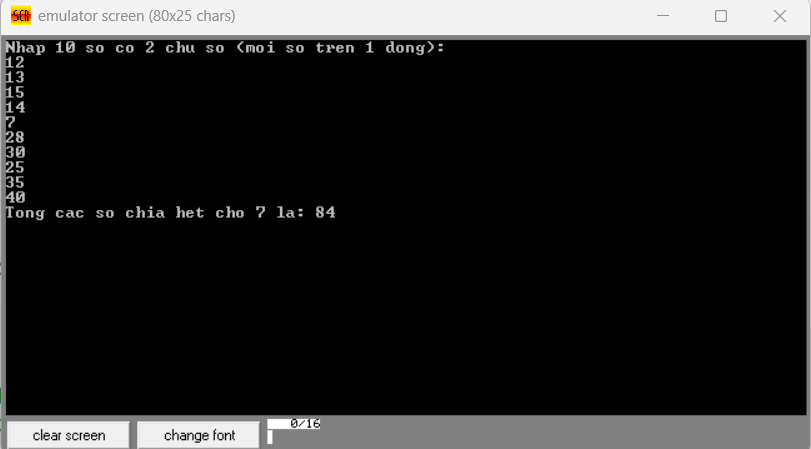
\includegraphics[width=0.8\textwidth]{Images/Result/B2.png}
    \caption{Giao diện hiển thị câu 2}
    \label{fig:result-2}
\end{figure}

